\section*{Exercise 6 Markov chain Monte-Carlo (Comments by Qahir)}
For this exercise we set $A_1,A_2=4$ and $n=10$. On table \ref{tab:tabex6} the $\chi^2$-test for the different MCMC-methods can be seen. As default we ran $20000$ iterations, had a burn-in of $1000$ and only included each $100$ sample in order to avoid serial correlation. To get a reasonable result for coordinate-wise metropolis we have had to increase the burn-in to $40000$ and only include each $300$ sample. This is probably due to there being much more correlation here. In all cases our tests are not significantly different from the true distribution setting $\alpha=0.05$. The coordinate-wise Metropolis-Hastings has a much lower P-value than the other methods even when we added a bigger burn-in and more iterations between each sample being stored. We are also not even sure of convergence for this method which can be verified by running the script multiple times. For all the other methods the p-values are generally higher than $0.5$ but for the coordinate-wise Metropolis-Hastings it might happen that we do not converge at all and up with p-values very close to $0$. On figure \ref{fig:ex61} a $2$-dimensional histogram for the $2$-dimensional MCMC methods can be seen. Also included is the true distribution and we can again see that coordinate-wise Metropolis-Hastings fares the worst. After this section relevant comments to each MCMC method can be seen. 
\begin{table}[H]
    \centering
    \begin{tabular}{|l|l|l|} \hline
        Method & P-value & Df  \\ \hline
        Metropolis-Hastings $(n=1)$& 0.5644  & 10 \\ \hline
        Direct Metropolis & 0.942318 & 65 \\ \hline
        Coordinate Metropolis & 0.11065 & 65 \\ \hline
        Gibbs sampling & 0.885 & 65\\ \hline
    \end{tabular}
    \caption{$\chi^2$-test for different MCMC-methods. The degrees of freedom is given as the number of classes minus $1$.}
    \label{tab:tabex6}
\end{table}

\begin{figure}[H]
        \centering
        \begin{subfigure}[H]{0.475\textwidth}
            \centering
            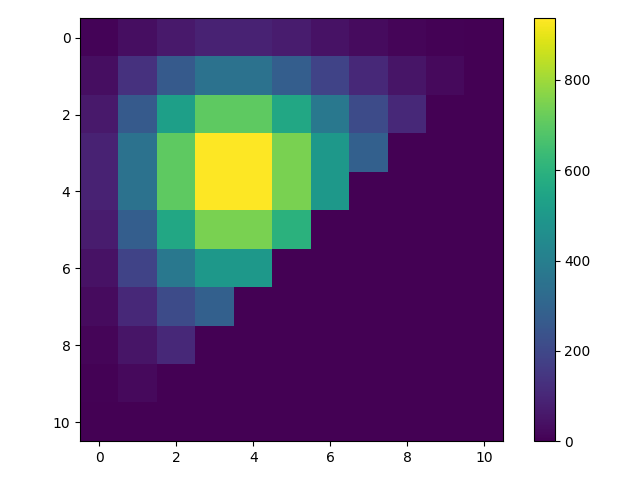
\includegraphics[width=\textwidth]{figures/true.png}
            \caption[Network2]%
            {{\small True distribution}}    
            \label{fig:mean and std of net14}
        \end{subfigure}
        \hfill
        \begin{subfigure}[H]{0.475\textwidth}  
            \centering 
            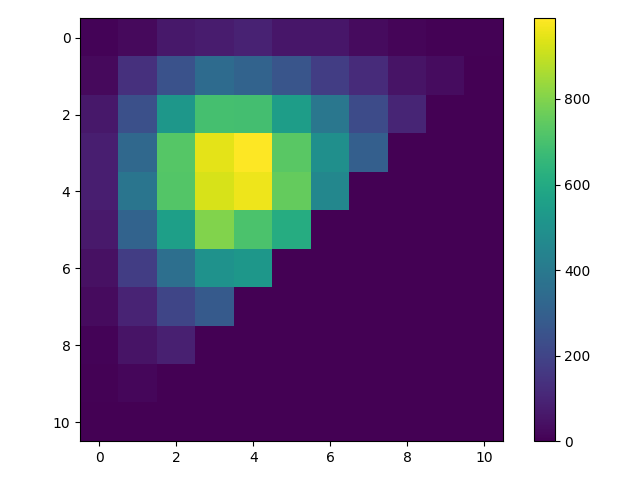
\includegraphics[width=\textwidth]{figures/direct.png}
            \caption[]%
            {{\small Gibbs}}    
            \label{fig:mean and std of net24}
        \end{subfigure}
        \vskip\baselineskip
        \begin{subfigure}[H]{0.475\textwidth}   
            \centering 
            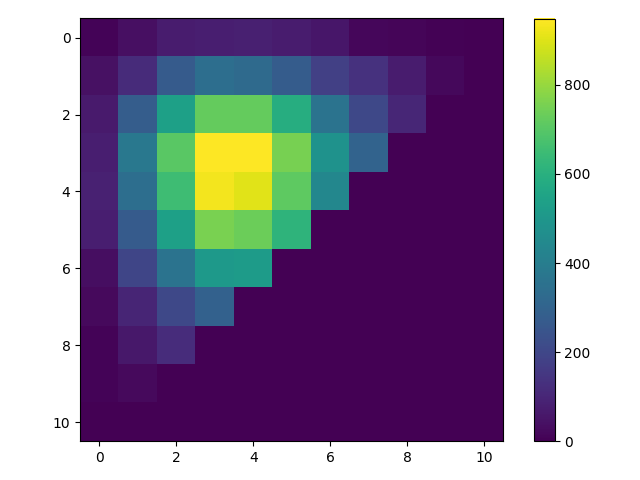
\includegraphics[width=\textwidth]{figures/gibbs.png}
            \caption[]%
            {{\small Direct Metropolis-Hastings}}    
            \label{fig:mean and std of net34}
        \end{subfigure}
        \quad
        \begin{subfigure}[H]{0.475\textwidth}   
            \centering 
            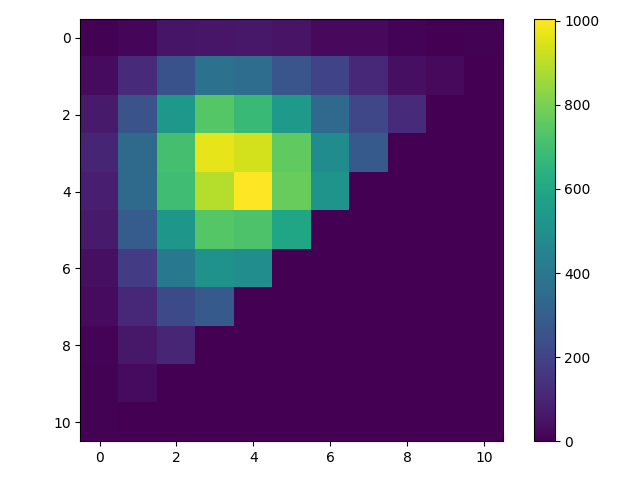
\includegraphics[width=\textwidth]{figures/coordinate.png}
            \caption[]%
            {{\small Coordinate-wise Metropolis-Hastings}}    
            \label{fig:stuff}
        \end{subfigure}
        \caption[ The average and standard deviation of critical parameters ]
        {\small $20000$ samples of different MCMC-methods. Also included is the true distribution. } 
        \label{fig:ex61}
    \end{figure}


\subsection*{Comments}

\subsubsection*{Metropolis-Hastings one dimensional case}
We would like to have a symmetric proposal distribution for ease of computation. This was done by setting the proposal jump from $X_i$ to $Y_i = \Delta X_i + X_i$ here we let $\Delta X_i \sim \text{Unif}(-1,1)$ (takes -1 and 1 as binary variables). Meaning we either go up or down. For the case where we are at the ends of the chain we simply connect $X_i=0$ and $X_j=n$ as can be seen on \ref{fig:ex62}. We of course used $n=10$, but $n=4$ was chosen for the figure and the concept easily generalizes to $n=10$. 


\begin{figure}[H]
    \centering
    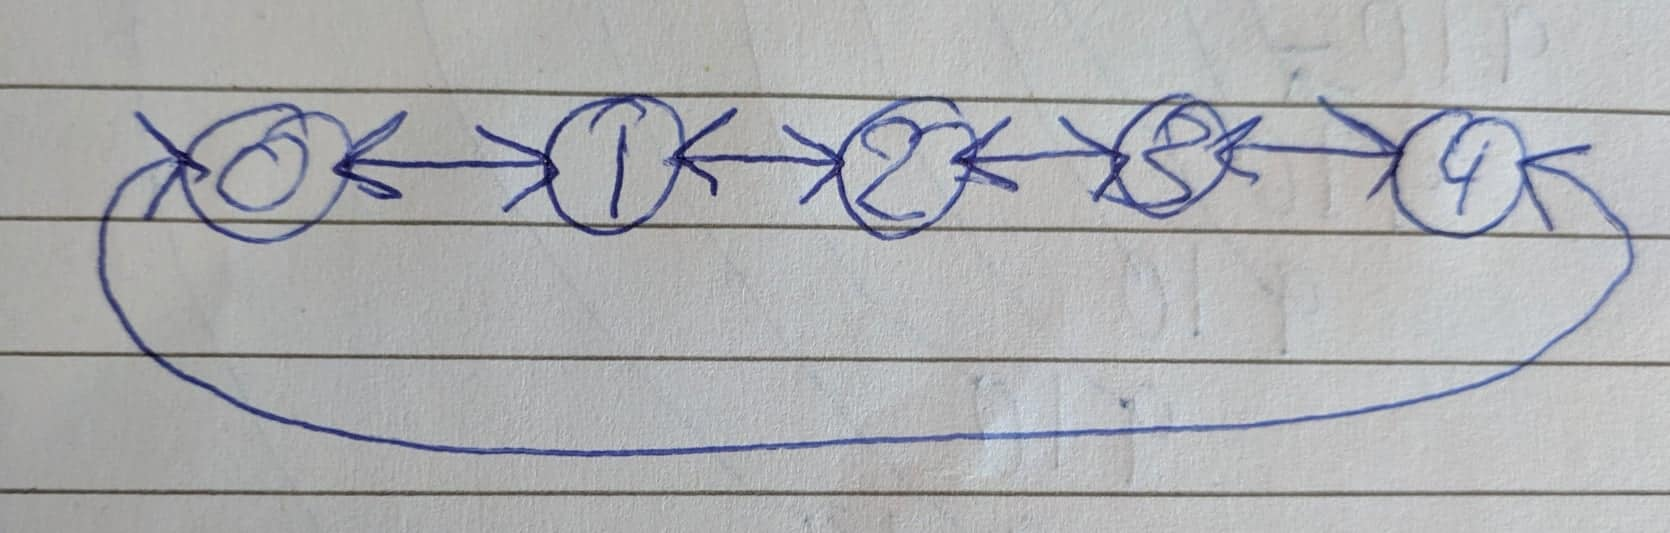
\includegraphics[width=\linewidth]{figures/pic2.jpg}
    \caption{Jumping performed for Metropolis-Hastings one dimension with $n=4$.}
    \label{fig:ex62}
\end{figure}

\subsection*{Metropolis-Hastings two-dimensional case}
We would like to have a symmetric proposal distribution. This was done by sampling $\Delta X_i \sim \text{Unif}(-1,0,1)$. We may end up at a point that is not part of the input space and in order to address this issue we perform the jumps seen on \ref{fig:ex62}. Performing the jumps like this ensures that the proposal distribution is symmetric. The number indicates the sum of both coordinates $X$ and $Y$. The figure shows what we do for $n=10$. When we are performing coordinate-wise sampling for the Metropolis Hastings we simply do not include the diagonal crossings and the jumping procedure can easily be deduced from figure \ref{fig:ex62}. 

\begin{figure}[H]
    \centering
    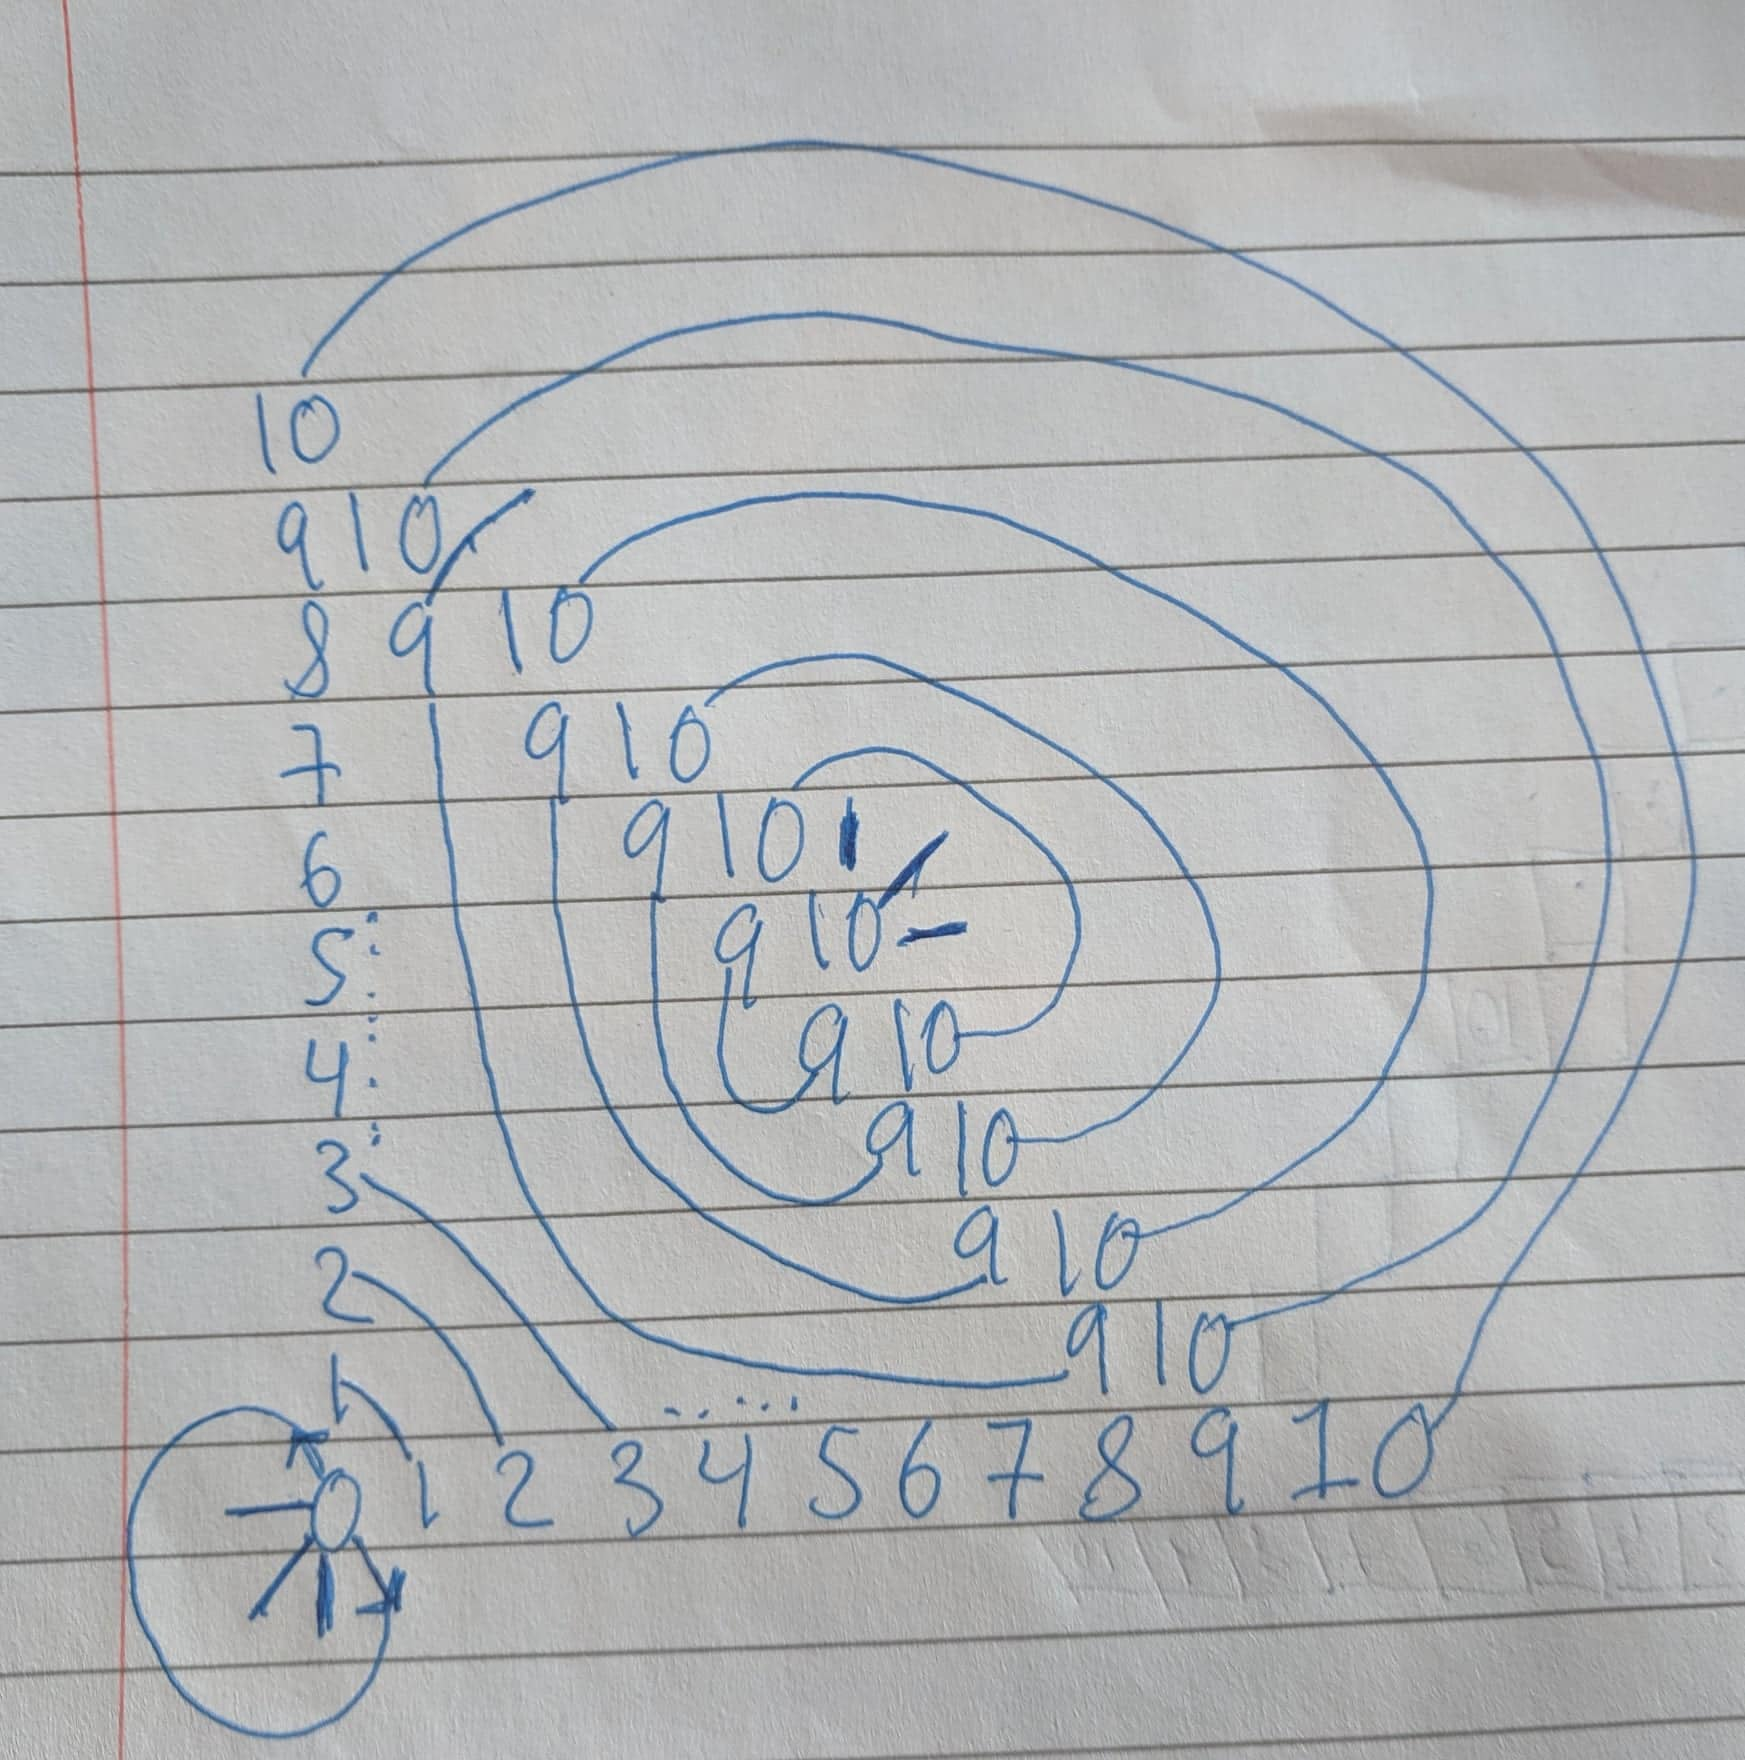
\includegraphics[width=\linewidth]{figures/pic1.jpg}
    \caption{Jumping performed for Metropolis-Hastings when booth coordinates are updated simultaneously. The jumping procedure for when one coordinate is updated each at a time can easily be deduced from this by simply removing diagonal jumps.}
    \label{fig:ex62}
\end{figure}


\subsubsection*{Normalization constant for $\chi^2$-test}
In order to perform the $\chi^2$-test we need the analytic form of the distribution and for this we need to determine the normalization constant. The normalization constant can be calculated as follows from summing over $\frac{4^i4^j}{j!i!}$ over the entire outcome space with the constraint $0 \leq j + i \leq 10$:

$$
K = \sum_{j,i, 0 \leq j+i \leq 10}\frac{4^i4^j}{j!i!}  =  \sum_{j=0}^{10}\sum_{i=0}^{10-j}\frac{4^i4^j}{j!i!} = \frac{3830591}{1575}
$$


\subsubsection*{Gibbs sampling}
First the conditional distribution is calculated by use of the rule $P(X)= \sum_{Y}P(X,Y)$ and $P(X|Y) = P(X,Y)/P(Y)$.  Due to the constraint $0 \leq j + i \leq 10$ it will have the following form:


$$
P(i|j) = \frac{P(i,j)}{P(j)} = \frac{\frac{1}{K}\frac{4^i 4^j}{i!j!}}{\frac{1}{K}\sum_{i'=0}^{10-j}\frac{4^{i'} 4^j}{i'!j!}} = \frac{\frac{4^i}{i!}}{\sum_{i'=0}^{10-j}\frac{4^{i'}}{i'!}}
$$

Due to symmetry one will have the exact same distribution for $P(j|i)$ just with $j$ and $i$ interchanged. We will Gibbs sample by iterating draws of $P(i|j)$ and then $P(j|i)$ - updating each coordinate at a time. To make draws of the conditional distributions we use the following theorem: Let $F$ denote the c.d.f of the stochastic variable we wish to sample and let $U \sim \text{unif}(0,1)$ then samples of the stochastic variable we wish to sample can be generated as $F^{-1}(U)$. In this case calculating $F$ and $F^{-1}$ is easy since we have a finite output space consisting of $66$ different combinations of $i$ and $j$. Sampling this way is also what was termed the crude method in the beginning of the course. 

% \subsection*{Comments by Sen}